\documentclass[aspectratio=169,8pt]{beamer}  % Reduced base font size to 8pt

% Theme settings
\usetheme{metropolis}
\usefonttheme{professionalfonts}
\usepackage[utf8]{inputenc}
\usepackage{graphicx}
\usepackage{amsmath}
\usepackage{booktabs}

% Title info
\title{Visual Intelligence: Lung Cancer Histopathological Classification}
\author{Lorenzo Mioso}
\date{March 2025}

\begin{document}

% Title slide
\begin{frame}
\titlepage
\end{frame}

% Introduction slide with adjusted image alignment
\begin{frame}{Introduction \& Problem Statement}
\begin{columns}[T]
\begin{column}{0.5\textwidth}
\begin{itemize}
\item \textbf{Dataset}: Lung cancer histopathological images (3 classes):
  \begin{itemize}
  \item \emph{Adenocarcinoma}
  \item \emph{Squamous cell carcinoma}
  \item \emph{Benign tissue}
  \end{itemize}
\item \textbf{Classification Task}: \emph{Binary classification} (adenocarcinoma vs benign tissue)
\item \textbf{Challenge}: Distinguishing \emph{subtle tissue patterns} and \emph{cellular structures}
\end{itemize}
\end{column}
\begin{column}{0.5\textwidth}
\hfill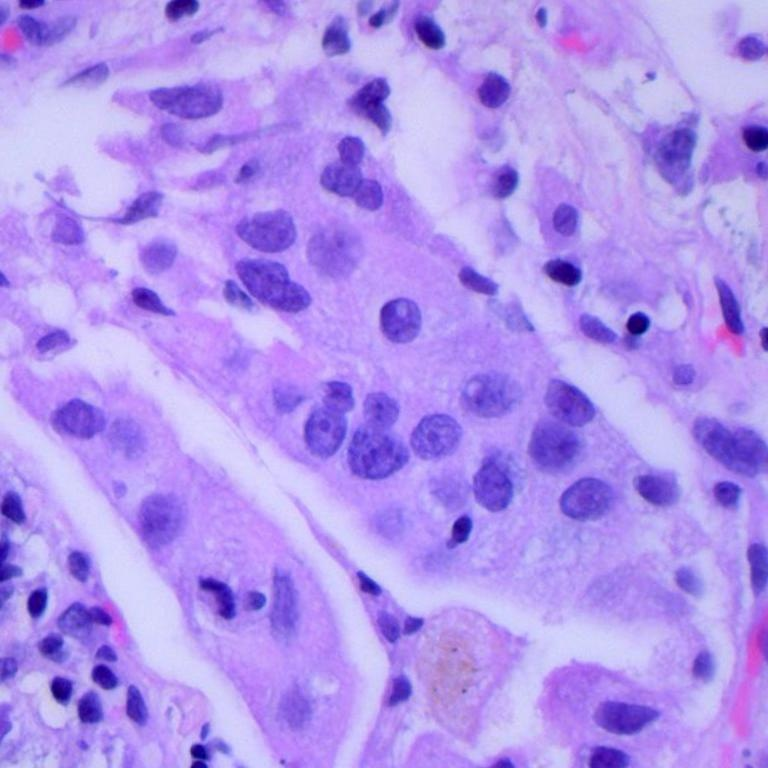
\includegraphics[width=0.95\linewidth, height=0.45\textheight]{imgs/adenocarcinoma.jpg}
\vspace{0.2cm}
\hfill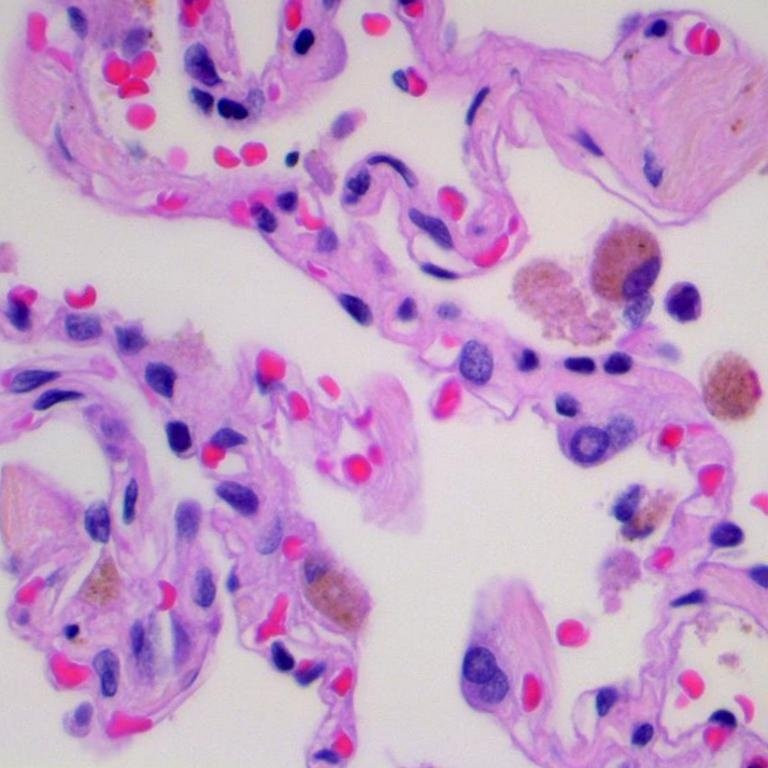
\includegraphics[width=0.95\linewidth, height=0.45\textheight]{imgs/benign.jpg}
\end{column}
\end{columns}
\end{frame}

% Project Goals slide
\begin{frame}{Project Goals}
\begin{itemize}
\item Compare \emph{traditional CNN} vs \emph{ScatNet} approaches (in particular for feature extraction)
\item Achieve \emph{high accuracy} with \emph{interpretable results}
\item Apply \emph{explainable AI techniques} to validate model decisions, in particular:
  \begin{itemize}
  \item \emph{Attribution analysis} with \emph{guided backpropagation} 
  \item \emph{Filter analysis} to understand learned patterns
  \end{itemize}
\end{itemize}
\end{frame}

% Data Preprocessing slide
\begin{frame}{Data Preprocessing \& Setup}
\begin{columns}[T]
\begin{column}{0.6\textwidth}
\begin{itemize}
\item \emph{Dataset Organization}:
  \begin{itemize}
  \item \emph{K-fold cross-validation} with 10 folds
  \item Class distributions already balanced
  \item Image size kept at \emph{768×768 pixels}
  \item \emph{Grayscale conversion} for analysis
  \end{itemize}
\end{itemize}

\begin{alertblock}{Key Finding}
Using grayscale images for analysis because with only color images, the model achieved high accuracy by learning \emph{color distributions}
\end{alertblock}
\end{column}
\begin{column}{0.4\textwidth}
\begin{figure}
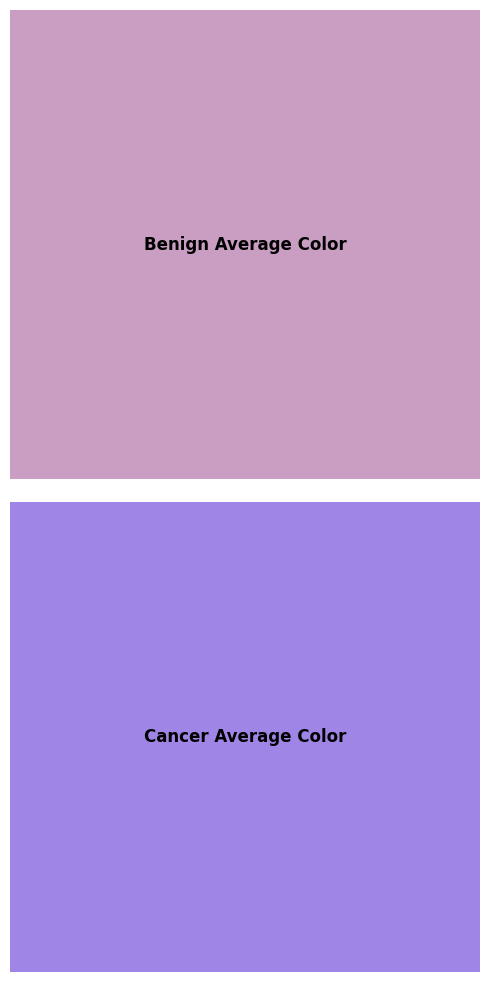
\includegraphics[width=0.7\textwidth, height=0.70\textheight]{imgs/class_avg_colors.png}
\end{figure}
\end{column}
\end{columns}
\end{frame}

% Preprocessing Pipeline slide with adjusted image alignment
\begin{frame}{Preprocessing Pipeline}
\begin{columns}[T]
\begin{column}{0.5\textwidth}
\begin{itemize}
\item Image \emph{normalization} and \emph{standardization} for each fold
\item The dataset already includes augmentation, but I added some more:
  \begin{itemize}
  \item \emph{Random rotations}
  \item \emph{Random flips}
  \item \emph{Color jittering}
  \item \emph{Random cropping}
  \item \emph{Gaussian noise}
  \end{itemize}
\end{itemize}
\end{column}
\begin{column}{0.5\textwidth}
\hfill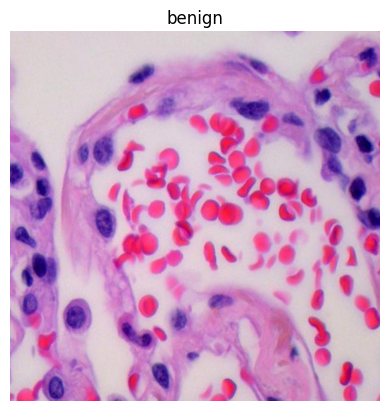
\includegraphics[width=0.95\linewidth, height=0.45\textheight]{imgs/normal_image.png}
\vspace{0.2cm}
\hfill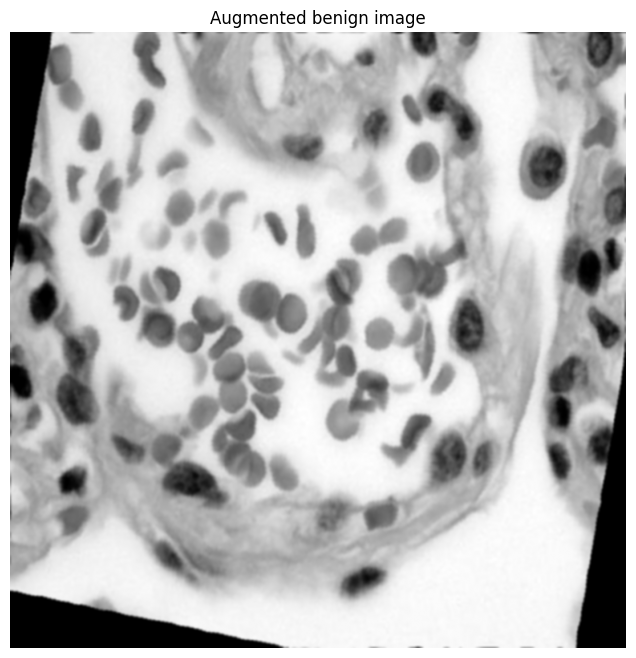
\includegraphics[width=0.95\linewidth, height=0.45\textheight]{imgs/augmented_image.png}
\end{column}
\end{columns}
\end{frame}

% CNN Model Architecture
\begin{frame}{CNN Model Architecture}
\begin{columns}[T]
\begin{column}{0.6\textwidth}
\begin{itemize}
\item \emph{Efficient Feature Extraction Design}:
  \begin{itemize}
  \item Similar to \emph{ResNet architecture} without skip connections
  \item Three progressive convolutional blocks (16→16→24 filters)
  \item First convolutional layer with \emph{11×11 kernel}
  \item Strategic dimensionality reduction via \emph{max pooling}
  \item \emph{Batch normalization} for improved training stability
  \item \emph{ReLU activations} for non-linear patterns
  \end{itemize}
\end{itemize}

\begin{alertblock}{Key Findings}
\begin{itemize}
\item Achieves \emph{exceptional classification accuracy} despite minimal parameters
\item First layer filters may not appear visually interpretable with small learning rates
\end{itemize}
\end{alertblock}
\end{column}
\begin{column}{0.4\textwidth}
\begin{figure}
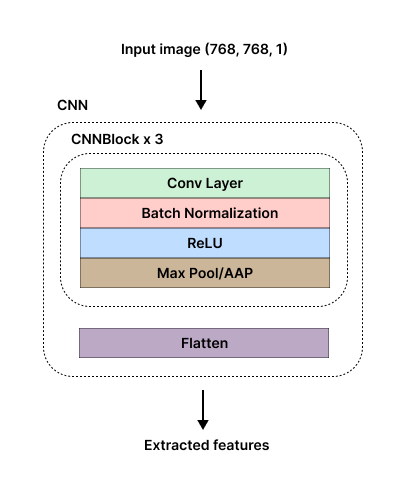
\includegraphics[width=0.9\textwidth]{imgs/cnn_arch.png}
\end{figure}
\end{column}
\end{columns}
\end{frame}

% Feature Classifier Architecture slide
\begin{frame}{Feature Classifier}
\begin{columns}[T]
\begin{column}{0.6\textwidth}
\begin{itemize}
\item Single hidden layer with 16 neurons
\item \emph{BatchNorm} for stability and faster convergence
\item \emph{ReLU activation} for non-linearity
\item \emph{Dropout (0.5)} for regularization
\item Final layer with 2 output neurons (softmax activation)
\end{itemize}
\end{column}
\begin{column}{0.4\textwidth}
\begin{figure}
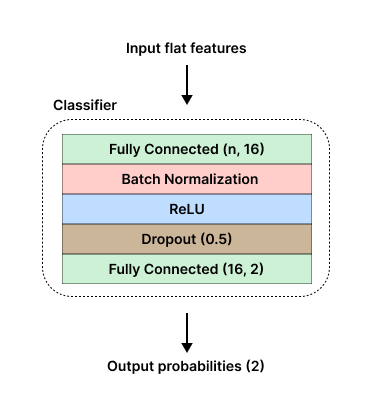
\includegraphics[width=\textwidth]{imgs/classifier_arch.png}
\end{figure}
\end{column}
\end{columns}
\end{frame}

% ScatNet Architecture slide
\begin{frame}{ScatNet Model Architecture}
\begin{columns}[T]
\begin{column}{0.6\textwidth}
\begin{itemize}
\item \textbf{Wavelet-based feature extraction}:
  \begin{itemize}
  \item \textbf{J=3} scale parameter for wavelet decomposition
  \item \textbf{L=8} orientations, \textbf{M=2} scattering order
  \item \textbf{Translation}, \textbf{rotation}, and \textbf{scaling invariant}
  \item Followed by global average pooling (4×4)
  \item 3,472 features fed to the classifier
  \end{itemize}
\end{itemize}

\begin{alertblock}{Key Finding}
Requires \textbf{more complex classifier} layer for good performance
\end{alertblock}
\end{column}
\begin{column}{0.4\textwidth}
\begin{figure}
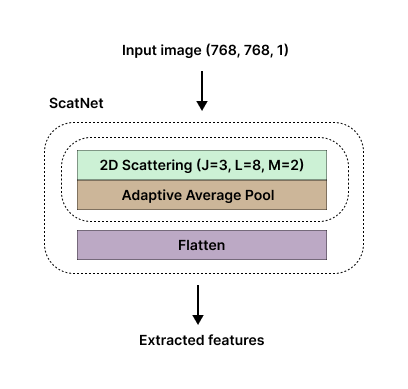
\includegraphics[width=\textwidth]{imgs/scatnet_arch.png}
\end{figure}
\end{column}
\end{columns}
\end{frame}

% Learning Curves Analysis slides
\begin{frame}{CNN Learning Curves Analysis}
\begin{columns}[T]
\begin{column}{0.5\textwidth}
\begin{itemize}
\item \textbf{Rapid convergence} within 15 epochs
\item \textbf{Consistent performance} across folds
\item \textbf{Limited overfitting} due to effective regularization
\item Final validation accuracy around \textbf{99\%}
\end{itemize}
\end{column}
\begin{column}{0.5\textwidth}
\begin{figure}
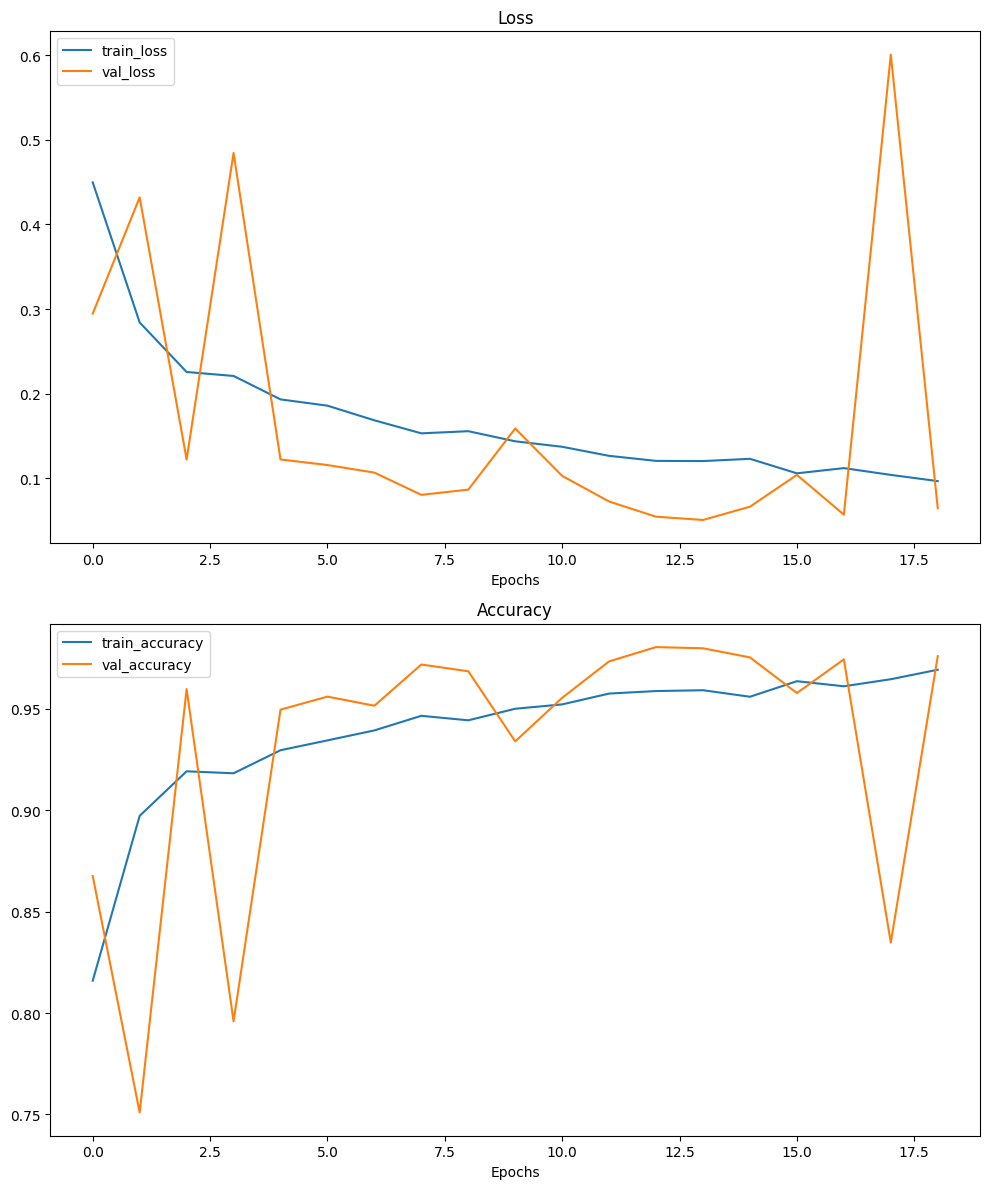
\includegraphics[width=\textwidth, height=0.9\textwidth]{imgs/cnn_train.png}
\end{figure}
\end{column}
\end{columns}
\end{frame}

\begin{frame}{ScatNet Learning Curves Analysis}
\begin{columns}[T]
\begin{column}{0.5\textwidth}
\begin{itemize}
\item \textbf{Slower convergence} but fewer epochs needed
\item \textbf{More complex classifier} needed
\item \textbf{Greater performance variation} across folds
\end{itemize}
\end{column}
\begin{column}{0.5\textwidth}
\begin{figure}
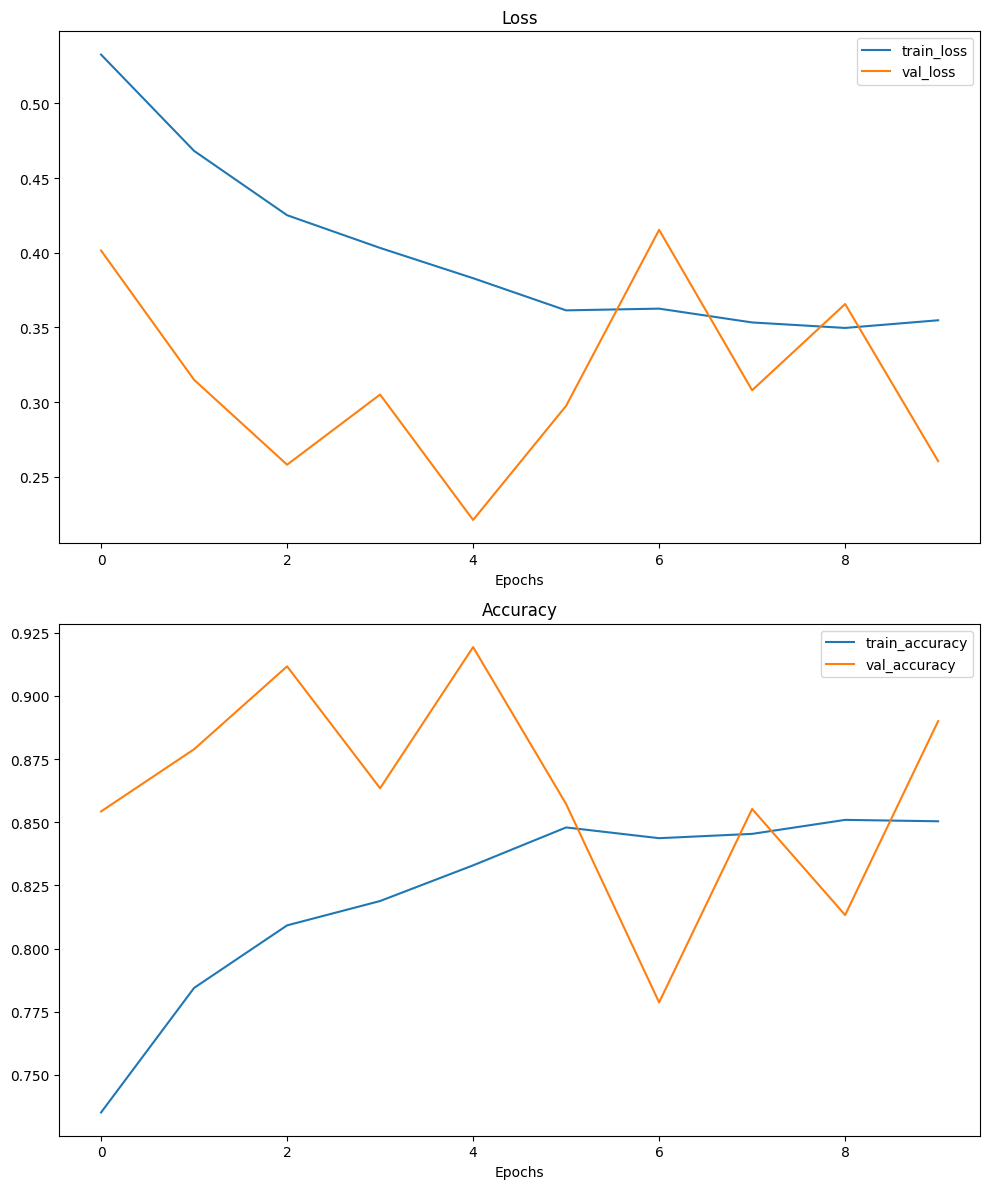
\includegraphics[width=\textwidth, height=0.9\textwidth]{imgs/scatnet_train.png}
\end{figure}
\end{column}
\end{columns}
\end{frame}

% Performance Results slide
\begin{frame}{Performance Results \& Analysis}
\begin{table}
\begin{tabular}{lll}
\toprule
Metric & \emph{CNN} & \emph{ScatNet} \\
\midrule
Mean Accuracy & \emph{99.26\% ± 0.72\%} & \emph{92.99\% ± 1.59\%} \\
Mean F1 Score & \emph{99.27\% ± 0.72\%} & \emph{92.83\% ± 1.70\%} \\
Accuracy Range & \emph{97.70\% - 99.90\%} & \emph{89.10\% - 95.10\%} \\
Training Speed & \emph{Faster} & \emph{Slower} \\
\bottomrule
\end{tabular}
\end{table}

\begin{alertblock}{Key Performance Findings}
\begin{itemize}
\item \emph{CNN significantly outperforms} ScatNet (by \emph{6.27\%})
\item \emph{K-fold validation} confirms \emph{robust performance}
\item \emph{CNN} shows \emph{less variance} between folds
\item \emph{CNN} achieves convergence in \emph{fewer epochs}
\end{itemize}
\end{alertblock}
\end{frame}

% Performance Summary slides
\begin{frame}{CNN Performance Summary}
\textbf{Performance Range:}
\begin{itemize}
\item Accuracy: \textbf{98.00\% - 99.90\%} across all folds
\item F1 Score: \textbf{98.01\% - 99.90\%} across all folds
\item Most consistent fold: \textbf{Fold 9} (99.90\% accuracy)
\item All folds achieved \textbf{\textgreater{}97.70\% accuracy}
\end{itemize}

\textbf{Overall Statistics:}
\begin{itemize}
\item Mean Accuracy: \textbf{99.26\%}
\item Mean F1 Score: \textbf{99.27\%}
\item Standard Deviation: \textbf{0.72\%}
\end{itemize}
\end{frame}

\begin{frame}{ScatNet Performance Summary}
\textbf{Performance Range:}
\begin{itemize}
\item Accuracy: \textbf{89.10\% - 95.10\%} across all folds
\item F1 Score: \textbf{88.68\% - 95.06\%} across all folds
\item Best performing fold: \textbf{Fold 6} (95.10\% accuracy)
\item Worst performing fold: \textbf{Fold 1} (89.10\% accuracy)
\end{itemize}

\textbf{Overall Statistics:}
\begin{itemize}
\item Mean Accuracy: \textbf{92.99\%}
\item Mean F1 Score: \textbf{92.83\%}
\item Standard Deviation: \textbf{1.59\%}
\end{itemize}
\end{frame}

% CNN Filter Analysis slides
\begin{frame}{CNN Filter Analysis}
\begin{columns}[T]
\begin{column}{0.6\textwidth}
\begin{itemize}
\item \textbf{Detected Filter Patterns}:
  \begin{itemize}
  \item \textbf{Diagonal/Vertical Strips}: Detect edges, gaps, and transitions between textures
  \item \textbf{Circular Points}: Identify spots, blobs, and localized features
  \item \textbf{Two-Part Filters}: Capture gradients and contrast changes
  \end{itemize}
\item \textbf{Filter Implications}:
  \begin{itemize}
  \item Learning localized and structured features
  \item Capturing directional patterns and contrast
  \item Detecting orientation-dependent structures
  \end{itemize}
\end{itemize}
\end{column}
\begin{column}{0.4\textwidth}
\begin{figure}
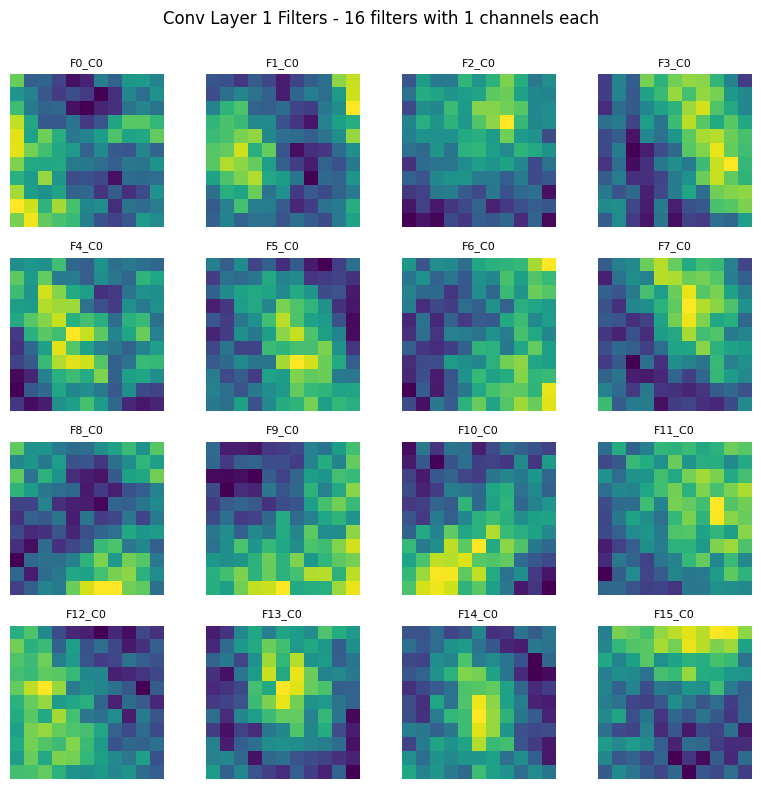
\includegraphics[width=\textwidth]{imgs/cnn_filters.png}
\end{figure}
\end{column}
\end{columns}
\end{frame}

% ScatNet Filter Analysis
\begin{frame}{ScatNet Filter Analysis}
\begin{columns}[T]
\begin{column}{0.5\textwidth}
\begin{itemize}
\item \textbf{Pre-defined wavelet transforms} (not learned)
\item \textbf{Scale and rotation invariant} features
\item \textbf{Lower discriminative power} despite theoretical advantages
\item Fixed mathematical representation \textbf{limits adaptability}
\item Data augmentation impact: \textbf{less significant}
\end{itemize}
\end{column}
\begin{column}{0.5\textwidth}
\begin{figure}
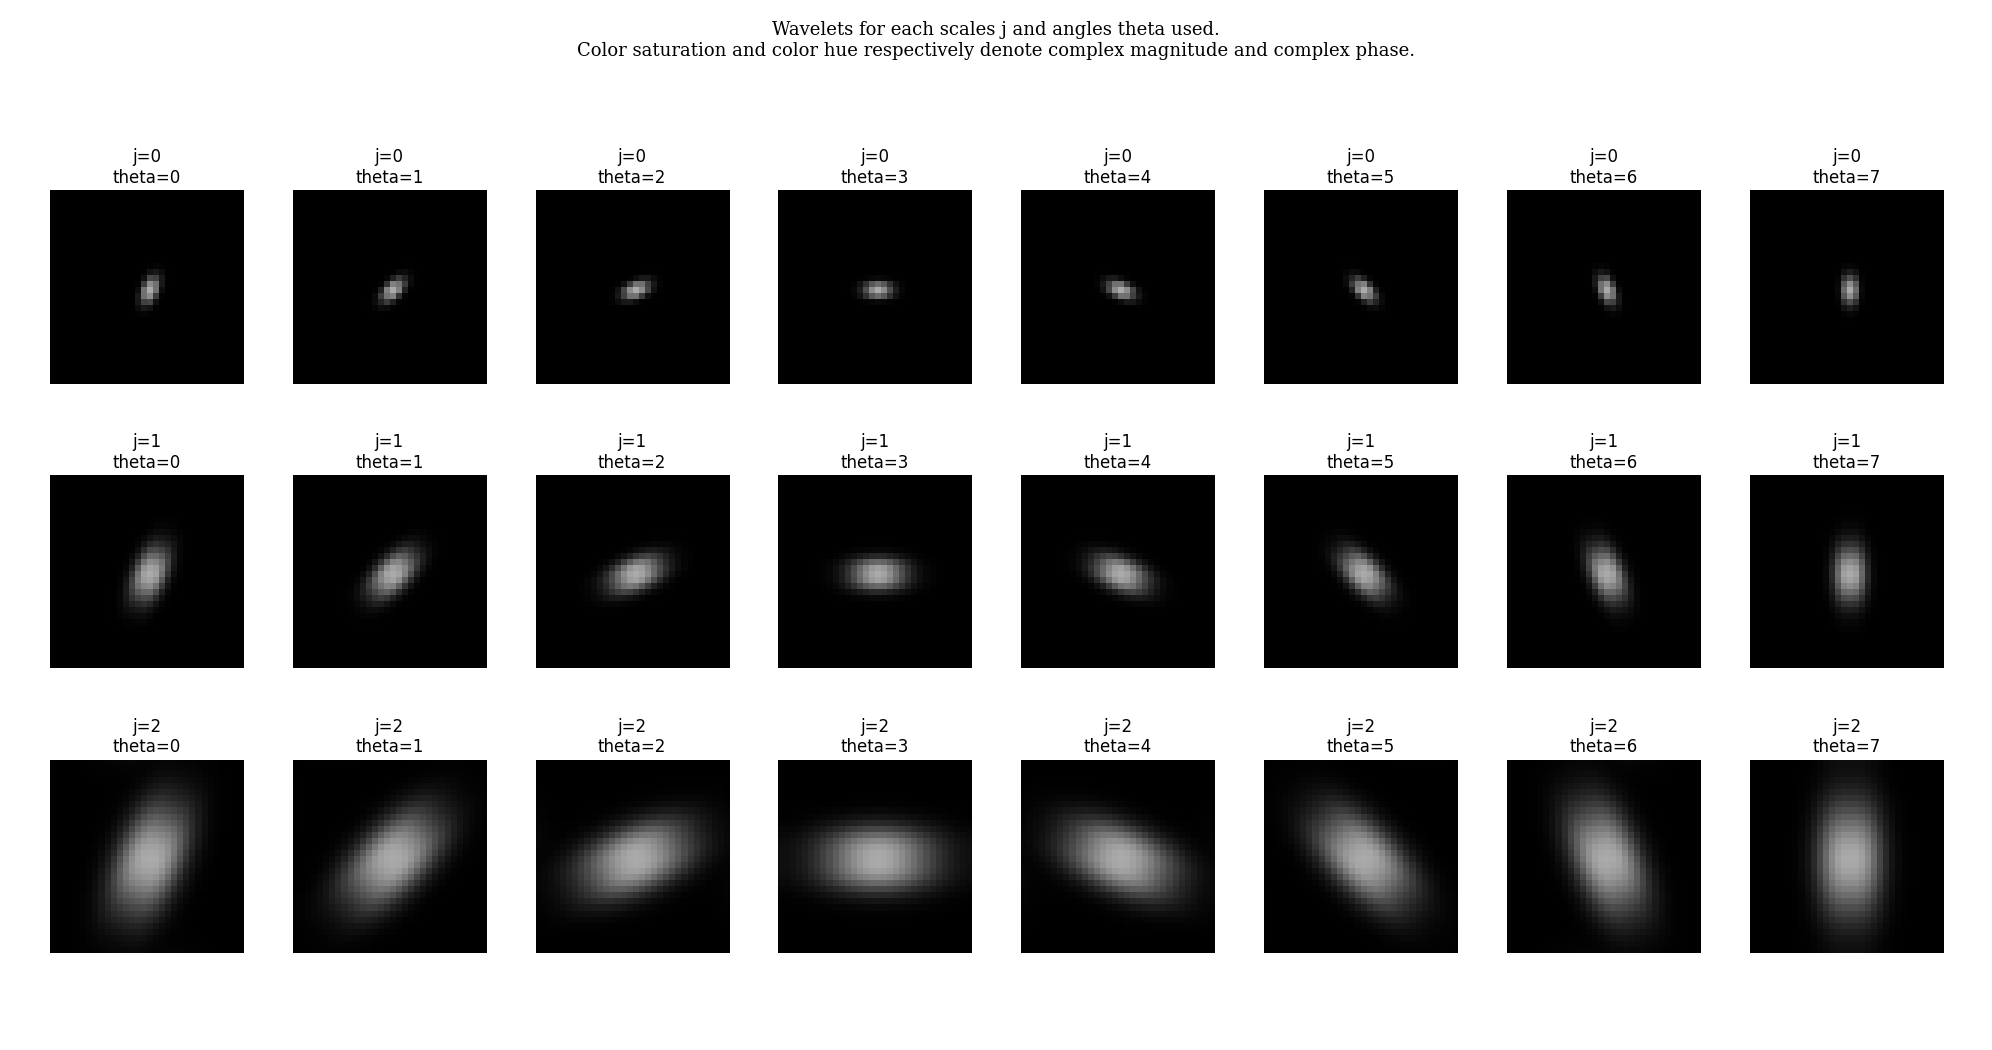
\includegraphics[width=0.7\textwidth]{imgs/scatnet_filters.png}
\vspace{0.5cm}
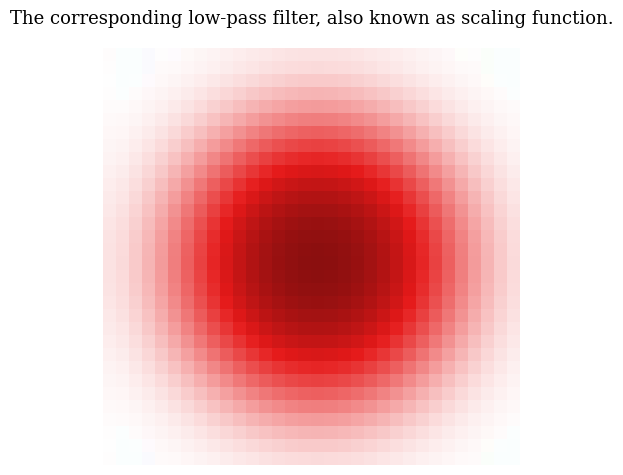
\includegraphics[width=0.7\textwidth]{imgs/scatnet_low_pass.png}
\end{figure}
\end{column}
\end{columns}
\end{frame}

% Attribution Analysis slides
\begin{frame}{CNN Attribution Analysis}
\begin{columns}[T]
\begin{column}{0.5\textwidth}
\begin{itemize}
\item Visualizes regions \textbf{most influential} for classification
\item \textbf{Guided backpropagation} significantly reduces noise compared to regular backpropagation
\item \textbf{Higher resolution} feature attribution with clearer patterns
\item Captum implementation shows \textbf{similar patterns} despite different color scaling
\item \textbf{Strong correlation} with pathological markers across all methods
\end{itemize}
\end{column}
\begin{column}{0.5\textwidth}
\begin{figure}
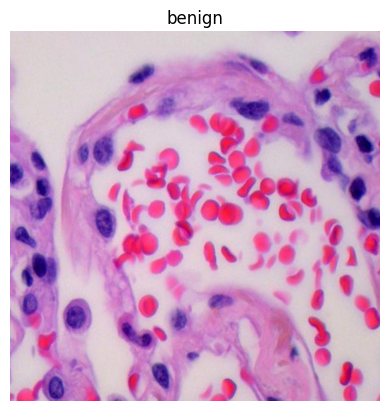
\includegraphics[width=0.45\textwidth]{imgs/normal_image.png}
\vspace{0.2cm}
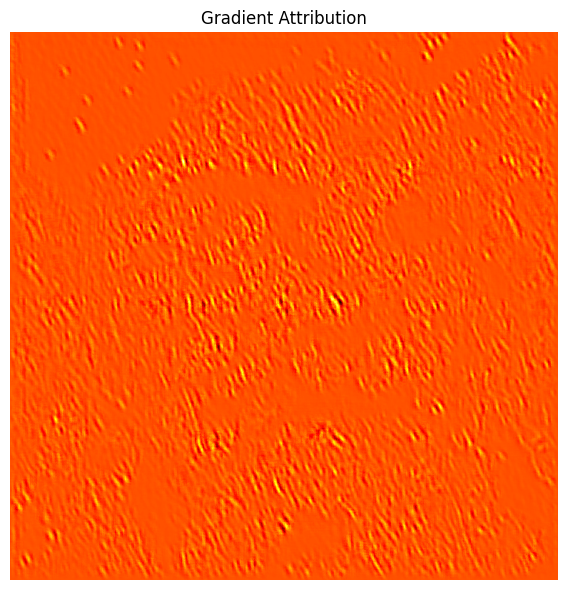
\includegraphics[width=0.45\textwidth]{imgs/cnn_bp.png}
\vspace{0.2cm}
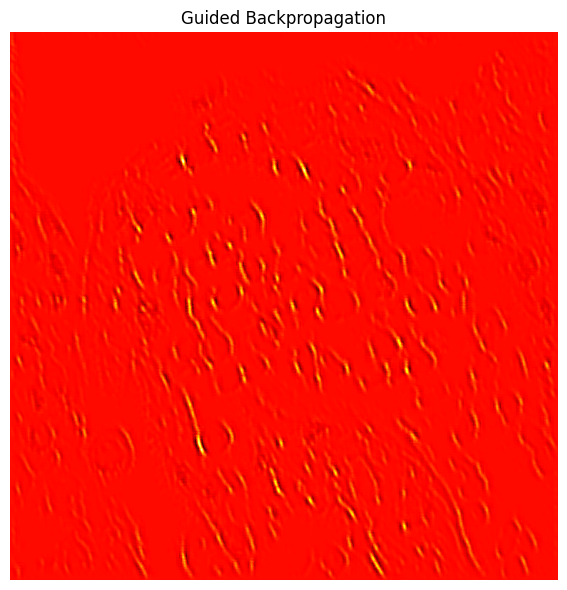
\includegraphics[width=0.45\textwidth]{imgs/cnn_gbp.png}
\vspace{0.2cm}
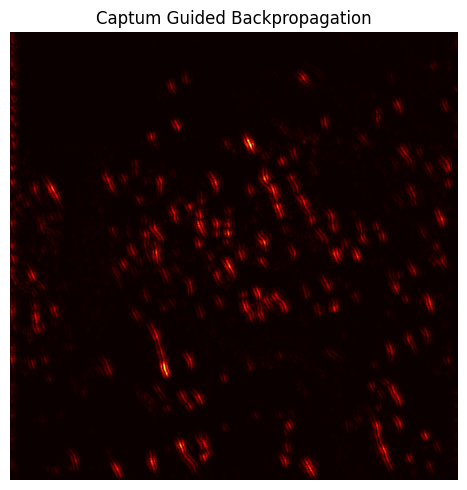
\includegraphics[width=0.45\textwidth]{imgs/cnn_gbp_captum.png}
\end{figure}
\end{column}
\end{columns}
\end{frame}

\begin{frame}{ScatNet Attribution Analysis}
\begin{columns}[T]
\begin{column}{0.5\textwidth}
\begin{itemize}
\item \textbf{Minimal differences} between guided and regular backpropagation
\item Limited impact of guided backprop due to \textbf{ReLU only in classifier}
\item \textbf{Non-recognizable patterns} in guided backprop visualization
\item Attribution shows \textbf{diffuse, less interpretable regions}
\item \textbf{Less coherent} with pathological indicators
\end{itemize}
\end{column}
\begin{column}{0.5\textwidth}
\begin{figure}
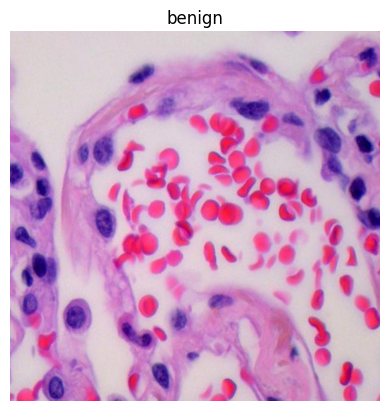
\includegraphics[width=0.45\textwidth]{imgs/normal_image.png}
\vspace{0.2cm}
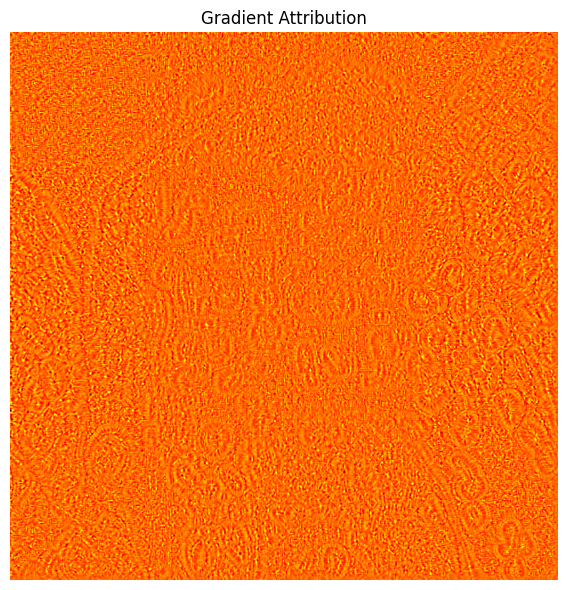
\includegraphics[width=0.45\textwidth]{imgs/scatnet_bp.png}
\vspace{0.2cm}
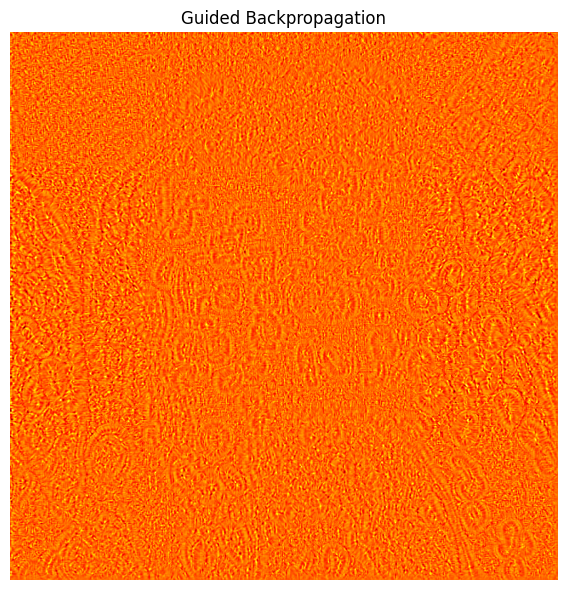
\includegraphics[width=0.45\textwidth]{imgs/scatnet_gbp.png}
\vspace{0.2cm}
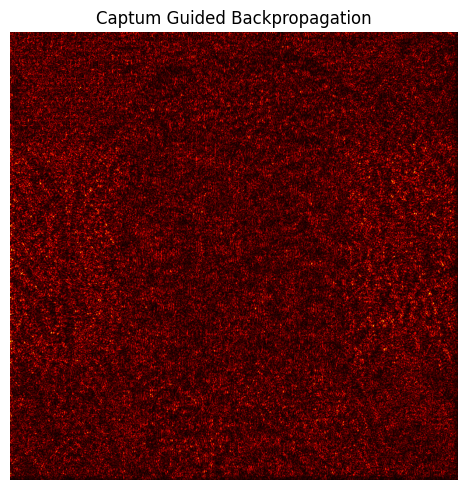
\includegraphics[width=0.45\textwidth]{imgs/scatnet_gbp_captum.png}
\end{figure}
\end{column}
\end{columns}
\end{frame}


% Key Insights slide
\begin{frame}{Key Insights}
\begin{itemize}
\item \emph{Color features} are not crucial for lung cancer histopathology classification
\item \emph{Learned features} (CNN), in this scenario, are more effective than \emph{pre-defined features} (ScatNet)
\item \emph{CNN} is harder to train but yields \emph{better performance}
\end{itemize}
\end{frame}

% Final slide
\begin{frame}[plain]
\centering
\vspace{2cm}
{\Large Thank you for your attention}

\vspace{1cm}
{\large Lorenzo Mioso}
\end{frame}

\end{document}